%%
%% Automatically generated file from DocOnce source
%% (https://github.com/hplgit/doconce/)
%%

% #define PREAMBLE

% #ifdef PREAMBLE
%-------------------- begin preamble ----------------------

\documentclass[%
oneside,                 % oneside: electronic viewing, twoside: printing
final,                   % draft: marks overfull hboxes, figures with paths
10pt]{article}

\listfiles               % print all files needed to compile this document

\usepackage{relsize,makeidx,color,setspace,amsmath,amsfonts,amssymb}
\usepackage[table]{xcolor}
\usepackage{bm,microtype}

\usepackage[pdftex]{graphicx}

% Packages for typesetting blocks of computer code
\usepackage{fancyvrb,framed,moreverb}

% Define colors
\definecolor{orange}{cmyk}{0,0.4,0.8,0.2}
\definecolor{tucorange}{rgb}{1.0,0.64,0}
\definecolor{darkorange}{rgb}{.71,0.21,0.01}
\definecolor{darkgreen}{rgb}{.12,.54,.11}
\definecolor{myteal}{rgb}{.26, .44, .56}
\definecolor{gray}{gray}{0.45}
\definecolor{mediumgray}{gray}{.8}
\definecolor{lightgray}{gray}{.95}
\definecolor{brown}{rgb}{0.54,0.27,0.07}
\definecolor{purple}{rgb}{0.5,0.0,0.5}
\definecolor{darkgray}{gray}{0.25}
\definecolor{darkblue}{rgb}{0,0.08,0.45}
\definecolor{darkblue2}{rgb}{0,0,0.8}
\definecolor{lightred}{rgb}{1.0,0.39,0.28}
\definecolor{lightgreen}{rgb}{0.48,0.99,0.0}
\definecolor{lightblue}{rgb}{0.53,0.81,0.92}
\definecolor{lightblue2}{rgb}{0.3,0.3,1.0}
\definecolor{lightpurple}{rgb}{0.87,0.63,0.87}
\definecolor{lightcyan}{rgb}{0.5,1.0,0.83}

\colorlet{comment_green}{green!50!black}
\colorlet{string_red}{red!60!black}
\colorlet{keyword_pink}{magenta!70!black}
\colorlet{indendifier_green}{green!70!white}

% Backgrounds for code
\definecolor{cbg_gray}{rgb}{.95, .95, .95}
\definecolor{bar_gray}{rgb}{.92, .92, .92}

\definecolor{cbg_yellowgray}{rgb}{.95, .95, .85}
\definecolor{bar_yellowgray}{rgb}{.95, .95, .65}

\colorlet{cbg_yellow2}{yellow!10}
\colorlet{bar_yellow2}{yellow!20}

\definecolor{cbg_yellow1}{rgb}{.98, .98, 0.8}
\definecolor{bar_yellow1}{rgb}{.98, .98, 0.4}

\definecolor{cbg_red1}{rgb}{1, 0.85, 0.85}
\definecolor{bar_red1}{rgb}{1, 0.75, 0.85}

\definecolor{cbg_blue1}{rgb}{0.87843, 0.95686, 1.0}
\definecolor{bar_blue1}{rgb}{0.7,     0.95686, 1}

%\setlength{\fboxsep}{-1.5mm}  % adjust cod_vpad/pro_vpad background box

%% Background for code blocks (parameter is color name)

%% pro/cod_vpad: gives some vertical padding before and after the text
%% (but has more simplistic code than _cod/pro_tight+cod/pro).
%% pro/cod_vpad can be used to enclose Verbatim or lst begin/end for code.
%% pro/cod calls _pro/cod_tight and has very little vertical padding,
%% used to enclose Verbatim and other begin/end for code.
%% (pro/cod is what the ptex2tex program could produce with the
%% Blue/BlueBar definitions in .ptex2tex.cfg.)

\newenvironment{cod_vpad}[1]{
   \def\FrameCommand{\colorbox{#1}}
   \MakeFramed{\FrameRestore}}
   {\endMakeFramed}

\newenvironment{_cod_tight}[1]{
   \def\FrameCommand{\colorbox{#1}}
   \FrameRule0.6pt\MakeFramed {\FrameRestore}\vskip3mm}
   {\vskip0mm\endMakeFramed}

\newenvironment{cod}[1]{
\bgroup\rmfamily
\fboxsep=0mm\relax
\begin{_cod_tight}{#1}
\list{}{\parsep=-2mm\parskip=0mm\topsep=0pt\leftmargin=2mm
\rightmargin=2\leftmargin\leftmargin=4pt\relax}
\item\relax}
{\endlist\end{_cod_tight}\egroup}

%% Background for complete program blocks (parameter 1 is color name
%% for background, parameter 2 is color for left bar)
\newenvironment{pro_vpad}[2]{
   \def\FrameCommand{\color{#2}\vrule width 1mm\normalcolor\colorbox{#1}}
   \MakeFramed{\FrameRestore}}
   {\endMakeFramed}

\newenvironment{_pro_tight}[2]{
   \def\FrameCommand{\color{#2}\vrule width 1mm\normalcolor\colorbox{#1}}
   \FrameRule0.6pt\MakeFramed {\advance\hsize-2mm\FrameRestore}\vskip3mm}
   {\vskip0mm\endMakeFramed}

\newenvironment{pro}[2]{
\bgroup\rmfamily
\fboxsep=0mm\relax
\begin{_pro_tight}{#1}{#2}
\list{}{\parsep=-2mm\parskip=0mm\topsep=0pt\leftmargin=2mm
\rightmargin=2\leftmargin\leftmargin=4pt\relax}
\item\relax}
{\endlist\end{_pro_tight}\egroup}

\usepackage{listingsutf8}

% Common lstlisting parameters
\lstset{
  basicstyle=\small \ttfamily,
  breaklines=false,          % break/wrap lines
  breakatwhitespace=true,    % let linebreaks happen at whitespace
  breakindent=40pt,
  tab=,
  tabsize=4,                 % tab means 4 spaces
  %belowskip=\smallskipamount,  % space between code and text below
  xleftmargin=5pt,           % indentation of code frame
  xrightmargin=5pt,
  framexleftmargin=5pt,      % add frame space to the left of code
  %numbers=left,             % put line numbers on the left
  %stepnumber=2,             % stepnumber=1 numbers each line, =n every n lines
  %framerule=0.4pt           % thickness of frame
  aboveskip=2ex,             % vertical space above code frame
  showstringspaces=false,    % show spaces in strings with an underscore
  showspaces=false,          % show spaces with an underscore
  showtabs=false,
  keepspaces=true,
  columns=fullflexible,      % tighter character kerning, like verb
  escapeinside={||},         % for |\pause| in slides and math in code blocks
  extendedchars=\true,       % allows non-ascii chars, does not work with utf-8
}

% Internally defined styles for lstlisting

\lstdefinestyle{simple}{
commentstyle={},
}

% end of custom lstdefinestyles

\usepackage[T1]{fontenc}
%\usepackage[latin1]{inputenc}
\usepackage{ucs}
\usepackage[utf8x]{inputenc}

\usepackage{lmodern}         % Latin Modern fonts derived from Computer Modern

% Hyperlinks in PDF:
\definecolor{linkcolor}{rgb}{0,0,0.4}
\usepackage{hyperref}
\hypersetup{
    breaklinks=true,
    colorlinks=true,
    linkcolor=linkcolor,
    urlcolor=linkcolor,
    citecolor=black,
    filecolor=black,
    %filecolor=blue,
    pdfmenubar=true,
    pdftoolbar=true,
    bookmarksdepth=3   % Uncomment (and tweak) for PDF bookmarks with more levels than the TOC
    }
%\hyperbaseurl{}   % hyperlinks are relative to this root

\setcounter{tocdepth}{2}  % number chapter, section, subsection

% Tricks for having figures close to where they are defined:
% 1. define less restrictive rules for where to put figures
\setcounter{topnumber}{2}
\setcounter{bottomnumber}{2}
\setcounter{totalnumber}{4}
\renewcommand{\topfraction}{0.95}
\renewcommand{\bottomfraction}{0.95}
\renewcommand{\textfraction}{0}
\renewcommand{\floatpagefraction}{0.75}
% floatpagefraction must always be less than topfraction!
% 2. ensure all figures are flushed before next section
\usepackage[section]{placeins}
% 3. enable begin{figure}[H] (often leads to ugly pagebreaks)
%\usepackage{float}\restylefloat{figure}

% prevent orhpans and widows
\clubpenalty = 10000
\widowpenalty = 10000

% --- end of standard preamble for documents ---


% insert custom LaTeX commands...

\raggedbottom
\makeindex
\usepackage[totoc]{idxlayout}   % for index in the toc
\usepackage[nottoc]{tocbibind}  % for references/bibliography in the toc

%-------------------- end preamble ----------------------

\begin{document}

% matching end for #ifdef PREAMBLE
% #endif

\newcommand{\half}{\frac{1}{2}}
\newcommand{\halfi}{{1/2}}
\newcommand{\tp}{\thinspace .}

\newcommand{\uex}{{u_{\small\mbox{e}}}}
\newcommand{\uexd}[1]{{u_{\small\mbox{e}, #1}}}
\newcommand{\vex}{{v_{\small\mbox{e}}}}
\newcommand{\vexd}[1]{{v_{\small\mbox{e}, #1}}}
\newcommand{\Aex}{{A_{\small\mbox{e}}}}

% Operators
\newcommand{\Ddt}[1]{\frac{D #1}{dt}}
\newcommand{\E}[1]{\hbox{E}\lbrack #1 \rbrack}
\newcommand{\Var}[1]{\hbox{Var}\lbrack #1 \rbrack}
\newcommand{\Std}[1]{\hbox{Std}\lbrack #1 \rbrack}

\newcommand{\xpoint}{\bm{x}}
\newcommand{\normalvec}{\bm{n}}
\newcommand{\Oof}[1]{\mathcal{O}(#1)}

% Boldface vectors/tensors
\newcommand{\x}{\bm{x}}
\newcommand{\X}{\bm{X}}
\renewcommand{\u}{\bm{u}}
\renewcommand{\v}{\bm{v}}
\newcommand{\w}{\bm{w}}
\newcommand{\acc}{\bm{a}}
\newcommand{\rpos}{\bm{r}}
\newcommand{\V}{\bm{V}}
\newcommand{\e}{\bm{e}}
\newcommand{\f}{\bm{f}}
\newcommand{\F}{\bm{F}}
\newcommand{\stress}{\bm{\sigma}}
\newcommand{\strain}{\bm{\varepsilon}}
\newcommand{\stressc}{{\sigma}}
\newcommand{\strainc}{{\varepsilon}}
\newcommand{\I}{\bm{I}}
\newcommand{\T}{\bm{T}}

\newcommand{\dfc}{\alpha}  % diffusion coefficient
% Unit vectors
\newcommand{\ii}{\bm{i}}
\newcommand{\jj}{\bm{j}}
\newcommand{\kk}{\bm{k}}
\newcommand{\ir}{\bm{i}_r}
\newcommand{\ith}{\bm{i}_{\theta}}
\newcommand{\iz}{\bm{i}_z}

% Index sets
\newcommand{\Ix}{\mathcal{I}_x}
\newcommand{\Iy}{\mathcal{I}_y}
\newcommand{\Iz}{\mathcal{I}_z}
\newcommand{\It}{\mathcal{I}_t}
%\newcommand{\Ix}{{I_x}}
%\newcommand{\Iy}{{I_y}}
%\newcommand{\Iz}{{I_z}}
%\newcommand{\It}{{I_t}}
%\newcommand{\If}{\mathcal{I}}     % for FEM
\newcommand{\If}{\mathcal{I}_s}     % for FEM
%\newcommand{\If}{{I}}     % for FEM
%\newcommand{\Ifd}{\mathcal{I}_d}  % for FEM
\newcommand{\Ifd}{{I_d}}  % for FEM
\newcommand{\Ifb}{{I_b}}  % for FEM
\newcommand{\setb}[1]{#1^0}    % set begin
\newcommand{\sete}[1]{#1^{-1}} % set end
%\newcommand{\setl}[1]{#1\setminus\{\set1{#1}\}}
%\newcommand{\setr}[1]{#1\setminus\{\set0{#1}\}}
%\newcommand{\seti}[1]{#1\setminus\{\set0{#1},\set1{#1}\}}
\newcommand{\setl}[1]{#1^-}
\newcommand{\setr}[1]{#1^+}
\newcommand{\seti}[1]{#1^i}
\newcommand{\sequencei}[1]{\left\{ {#1}_i \right\}_{i\in\If}}

% Finite elements
\newcommand{\basphi}{\varphi}
\newcommand{\baspsi}{\psi}
\newcommand{\refphi}{\tilde\basphi}
\newcommand{\psib}{\bm{\psi}}
\newcommand{\sinL}[1]{\sin\left((#1+1)\pi\frac{x}{L}\right)}
\newcommand{\xno}[1]{x_{#1}}
%\newcommand{\xno}[1]{x^{(#1)}}
\newcommand{\Xno}[1]{X_{(#1)}}
\newcommand{\yno}[1]{y_{#1}}
\newcommand{\Yno}[1]{Y_{(#1)}}
\newcommand{\xdno}[1]{\bm{x}_{#1}}

% FEniCS commands
\newcommand{\dX}{\, \mathrm{d}X}
\newcommand{\dx}{\, \mathrm{d}x}
\newcommand{\ds}{\, \mathrm{d}s}
\newcommand{\Real}{\mathbb{R}}
\newcommand{\Integerp}{\mathbb{N}}
\newcommand{\Integer}{\mathbb{Z}}


% ------------------- main content ----------------------



% ----------------- title -------------------------

\thispagestyle{empty}

\begin{center}
{\LARGE\bf
\begin{spacing}{1.25}
Study guide: Generalizations of exponential decay models
\end{spacing}
}
\end{center}

% ----------------- author(s) -------------------------

\begin{center}
{\bf Hans Petter Langtangen${}^{1, 2}$} \\ [0mm]
\end{center}

\begin{center}
% List of all institutions:
\centerline{{\small ${}^1$Center for Biomedical Computing, Simula Research Laboratory}}
\centerline{{\small ${}^2$Department of Informatics, University of Oslo}}
\end{center}
    
% ----------------- end author(s) -------------------------

% --- begin date ---
\begin{center}
Oct 10, 2015
\end{center}
% --- end date ---

\vspace{1cm}


% !split
\section*{Model extensions}
\label{decay:generalizations}

% !split
\subsection*{Extension to a variable coefficient; Forward and Backward Euler}

\begin{equation}
u'(t) = -a(t)u(t),\quad t\in (0,T],\quad u(0)=I
\label{decay:problem:a}
\end{equation}


The Forward Euler scheme:

\begin{equation}
\frac{u^{n+1} - u^n}{\Delta t} = -a(t_n)u^n
\end{equation}

The Backward Euler scheme:
\begin{equation}
\frac{u^{n} - u^{n-1}}{\Delta t} = -a(t_n)u^n
\end{equation}

% !split
\subsection*{Extension to a variable coefficient; Crank-Nicolson}

Eevaluting $a(t_{n+\half})$ and
using an average for $u$:
\begin{equation}
\frac{u^{n+1} - u^{n}}{\Delta t} = -a(t_{n+\half})\half(u^n + u^{n+1})
\end{equation}

Using an average for $a$ and $u$:
\begin{equation}
\frac{u^{n+1} - u^{n}}{\Delta t} = -\half(a(t_n)u^n + a(t_{n+1})u^{n+1})
\end{equation}

% !split
\subsection*{Extension to a variable coefficient; $\theta$-rule}

The $\theta$-rule unifies the three mentioned schemes,

\begin{equation}
\frac{u^{n+1} - u^{n}}{\Delta t} = -a((1-\theta)t_n + \theta t_{n+1})((1-\theta) u^n + \theta u^{n+1})
\end{equation}
or,
\begin{equation}
\frac{u^{n+1} - u^{n}}{\Delta t} = -(1-\theta) a(t_n)u^n - \theta
a(t_{n+1})u^{n+1}
\end{equation}

% !split
\subsection*{Extension to a variable coefficient; operator notation}

\begin{align*}
\lbrack D^+_t u &= -au\rbrack^n,\\ 
\lbrack D^-_t u &= -au\rbrack^n,\\ 
\lbrack D_t u &= -a\overline{u}^t\rbrack^{n+\half},\\ 
\lbrack D_t u &= -\overline{au}^t\rbrack^{n+\half}\\ 
\end{align*}


% !split
\subsection*{Extension to a source term}
\label{decay:source}

\begin{equation}
u'(t) = -a(t)u(t) + b(t),\quad t\in (0,T],\quad u(0)=I
\label{decay:problem:ab}
\end{equation}

\begin{align*}
\lbrack D^+_t u &= -au + b\rbrack^n,\\ 
\lbrack D^-_t u &= -au + b\rbrack^n,\\ 
\lbrack D_t u   &= -a\overline{u}^t + b\rbrack^{n+\half},\\ 
\lbrack D_t u   &= \overline{-au+b}^t\rbrack^{n+\half}
\end{align*}

% !split
\subsection*{Implementation of the generalized model problem}
\label{decay:general}

\begin{equation}
u^{n+1} = ((1 - \Delta t(1-\theta)a^n)u^n
+ \Delta t(\theta b^{n+1} + (1-\theta)b^n))(1 + \Delta t\theta a^{n+1})^{-1}
\end{equation}

Implementation where $a(t)$ and $b(t)$ are given as
Python functions (see file \href{{http://tinyurl.com/ofkw6kc/genz/decay_vc.py}}{\nolinkurl{decay_vc.py}}):

\begin{cod}{cbg_yellow2}\begin{lstlisting}[language=Python,style=simple,xleftmargin=2mm]
def solver(I, a, b, T, dt, theta):
    """
    Solve u'=-a(t)*u + b(t), u(0)=I,
    for t in (0,T] with steps of dt.
    a and b are Python functions of t.
    """
    dt = float(dt)            # avoid integer division
    Nt = int(round(T/dt))     # no of time intervals
    T = Nt*dt                 # adjust T to fit time step dt
    u = zeros(Nt+1)           # array of u[n] values
    t = linspace(0, T, Nt+1)  # time mesh

    u[0] = I                  # assign initial condition
    for n in range(0, Nt):    # n=0,1,...,Nt-1
        u[n+1] = ((1 - dt*(1-theta)*a(t[n]))*u[n] + \ 
                  dt*(theta*b(t[n+1]) + (1-theta)*b(t[n])))/\ 
                  (1 + dt*theta*a(t[n+1]))
    return u, t
\end{lstlisting}\end{cod}
\noindent

% !split
\subsection*{Implementations of variable coefficients; functions}

Plain functions:

\begin{cod}{cbg_yellow2}\begin{lstlisting}[language=Python,style=simple,xleftmargin=2mm]
def a(t):
    return a_0 if t < tp else k*a_0

def b(t):
    return 1
\end{lstlisting}\end{cod}
\noindent

% !split
\subsection*{Implementations of variable coefficients; classes}

Better implementation: class with the parameters \texttt{a0}, \texttt{tp}, and \texttt{k}
as attributes and a \emph{special method} \Verb!__call__! for evaluating $a(t)$:

\begin{cod}{cbg_yellow2}\begin{lstlisting}[language=Python,style=simple,xleftmargin=2mm]
class A:
    def __init__(self, a0=1, k=2):
        self.a0, self.k = a0, k

    def __call__(self, t):
        return self.a0 if t < self.tp else self.k*self.a0

a = A(a0=2, k=1)  # a behaves as a function a(t)
\end{lstlisting}\end{cod}
\noindent

% !split
\subsection*{Implementations of variable coefficients; lambda function}

\index{lambda functions}

Quick writing: a one-liner \emph{lambda function}
\begin{cod}{cbg_yellow2}\begin{lstlisting}[language=Python,style=simple,xleftmargin=2mm]
a = lambda t: a_0 if t < tp else k*a_0
\end{lstlisting}\end{cod}
\noindent

In general,
\begin{cod}{cbg_yellow2}\begin{lstlisting}[language=Python,style=simple,xleftmargin=2mm]
f = lambda arg1, arg2, ...: expressin
\end{lstlisting}\end{cod}
\noindent
is equivalent to
\begin{cod}{cbg_yellow2}\begin{lstlisting}[language=Python,style=simple,xleftmargin=2mm]
def f(arg1, arg2, ...):
    return expression
\end{lstlisting}\end{cod}
\noindent

One can use lambda functions directly in calls:
\begin{cod}{cbg_yellow2}\begin{lstlisting}[language=Python,style=simple,xleftmargin=2mm]
u, t = solver(1, lambda t: 1, lambda t: 1, T, dt, theta)
\end{lstlisting}\end{cod}
\noindent
for a problem $u'=-u+1$, $u(0)=1$.

A lambda function can appear anywhere where a variable can appear.

% !split
\subsection*{Verification via trivial solutions}
\label{decay:verify:trivial}

\begin{itemize}
 \item Start debugging of a new code with trying a problem
   where $u=\hbox{const} \neq 0$.

 \item Choose $u=C$ (a constant). Choose any $a(t)$ and set
   $b=a(t)C$ and
   $I=C$.

 \item "All" numerical methods will reproduce $u=_{\hbox{const}}$
   exactly (machine precision).

 \item Often $u=C$ eases debugging.

 \item In this example: \emph{any error} in the formula for $u^{n+1}$
   make $u\neq C$!
\end{itemize}

\noindent
% !split
\subsection*{Verification via trivial solutions; test function}

\begin{cod}{cbg_yellow2}\begin{lstlisting}[language=Python,style=simple,xleftmargin=2mm]
def test_constant_solution():
    """
    Test problem where u=u_const is the exact solution, to be
    reproduced (to machine precision) by any relevant method.
    """
    def u_exact(t):
        return u_const

    def a(t):
        return 2.5*(1+t**3)  # can be arbitrary

    def b(t):
        return a(t)*u_const

    u_const = 2.15
    theta = 0.4; I = u_const; dt = 4
    Nt = 4  # enough with a few steps
    u, t = solver(I=I, a=a, b=b, T=Nt*dt, dt=dt, theta=theta)
    print u
    u_e = u_exact(t)
    difference = abs(u_e - u).max()  # max deviation
    tol = 1E-14
    assert difference < tol
\end{lstlisting}\end{cod}
\noindent


% !split
\subsection*{Verification via manufactured solutions}
\label{decay:MMS}

\index{method of manufactured solutions}
\index{MMS (method of manufactured solutions)}

\begin{itemize}
 \item Choose \emph{any} formula for $u(t)$

 \item Fit $I$, $a(t)$, and $b(t)$ in $u'=-au+b$, $u(0)=I$,
   to make the chosen formula a solution of the ODE problem

 \item Then we can always have an analytical solution (!)

 \item Ideal for verification: testing convergence rates

 \item Called the \emph{method of manufactured solutions} (MMS)

 \item Special case: $u$ linear in $t$, because all sound numerical
   methods will reproduce a linear $u$ exactly (machine precision)

 \item $u(t) = ct + d$. $u(0)=0$ means $d=I$

 \item ODE implies $c = -a(t)u + b(t)$

 \item Choose $a(t)$ and $c$, and set $b(t) = c + a(t)(ct + I)$

 \item Any error in the formula for $u^{n+1}$ makes $u\neq ct+I$!
\end{itemize}

\noindent
% !split
\subsection*{Linear manufactured solution}

$u^n = ct_n+I$ fulfills the discrete
equations!

First,
\begin{align}
\lbrack D_t^+ t\rbrack^n &= \frac{t_{n+1}-t_n}{\Delta t}=1,
\label{decay:fd2:Dop:tn:fw}\\ 
\lbrack D_t^- t\rbrack^n &= \frac{t_{n}-t_{n-1}}{\Delta t}=1,
\label{decay:fd2:Dop:tn:bw}\\ 
\lbrack D_t t\rbrack^n &= \frac{t_{n+\half}-t_{n-\half}}{\Delta t}=\frac{(n+\half)\Delta t - (n-\half)\Delta t}{\Delta t}=1\label{decay:fd2:Dop:tn:cn}
\end{align}

Forward Euler:

\[ [D^+ u = -au + b]^n \]

$a^n=a(t_n)$, $b^n=c + a(t_n)(ct_n + I)$, and $u^n=ct_n + I$
results in

\[ c = -a(t_n)(ct_n+I) + c + a(t_n)(ct_n + I) = c \]

% !split
\subsection*{Test function for linear manufactured solution}

\begin{cod}{cbg_yellow2}\begin{lstlisting}[language=Python,style=simple,xleftmargin=2mm]
def test_linear_solution():
    """
    Test problem where u=c*t+I is the exact solution, to be
    reproduced (to machine precision) by any relevant method.
    """
    def u_exact(t):
        return c*t + I

    def a(t):
        return t**0.5  # can be arbitrary

    def b(t):
        return c + a(t)*u_exact(t)

    theta = 0.4; I = 0.1; dt = 0.1; c = -0.5
    T = 4
    Nt = int(T/dt)  # no of steps
    u, t = solver(I=I, a=a, b=b, T=Nt*dt, dt=dt, theta=theta)
    u_e = u_exact(t)
    difference = abs(u_e - u).max()  # max deviation
    print difference
    tol = 1E-14  # depends on c!
    assert difference < tol
\end{lstlisting}\end{cod}
\noindent

% !split
\section*{Computing convergence rates}
\label{decay:convrates}

Frequent assumption on the relation between the numerical error $E$ and
some discretization parameter $\Delta t$:

\begin{equation}
E = C\Delta t^r,
\label{decay:E:dt}
\end{equation}

\begin{itemize}
 \item Unknown: $C$ and $r$.

 \item Goal: estimate $r$ (and $C$) from numerical experiments
\end{itemize}

\noindent
% !split
\subsection*{Estimating the convergence rate $r$}

Perform numerical experiments: $(\Delta t_i, E_i)$, $i=0,\ldots,m-1$.
Two methods for finding $r$ (and $C$):

\begin{enumerate}
 \item Take the logarithm of (\ref{decay:E:dt}), $\ln E = r\ln \Delta t + \ln C$,
    and fit a straight line to the data points $(\Delta t_i, E_i)$,
    $i=0,\ldots,m-1$.

 \item Consider two consecutive experiments, $(\Delta t_i, E_i)$ and
    $(\Delta t_{i-1}, E_{i-1})$. Dividing the equation
    $E_{i-1}=C\Delta t_{i-1}^r$ by $E_{i}=C\Delta t_{i}^r$ and solving
    for $r$ yields
\end{enumerate}

\noindent
\begin{equation}
r_{i-1} = \frac{\ln (E_{i-1}/E_i)}{\ln (\Delta t_{i-1}/\Delta t_i)}
\label{decay:conv:rate}
\end{equation}
for $i=1,=\ldots,m-1$.

Method 2 is best.

% !split
\subsection*{Brief implementation}

Compute $r_0, r_1, \ldots, r_{m-2}$ from $E_i$ and $\Delta t_i$:

\begin{cod}{cbg_yellow2}\begin{lstlisting}[language=Python,style=simple,xleftmargin=2mm]
def compute_rates(dt_values, E_values):
    m = len(dt_values)
    r = [log(E_values[i-1]/E_values[i])/
         log(dt_values[i-1]/dt_values[i])
         for i in range(1, m, 1)]
    # Round to two decimals
    r = [round(r_, 2) for r_ in r]
    return r
\end{lstlisting}\end{cod}
\noindent

% !split
\subsection*{We embed the code in a real test function}

\begin{cod}{cbg_yellow2}\begin{lstlisting}[language=Python,style=simple,xleftmargin=2mm]
def test_convergence_rates():
    # Create a manufactured solution
    # define u_exact(t), a(t), b(t)

    dt_values = [0.1*2**(-i) for i in range(7)]
    I = u_exact(0)

    for theta in (0, 1, 0.5):
        E_values = []
        for dt in dt_values:
            u, t = solver(I=I, a=a, b=b, T=6, dt=dt, theta=theta)
            u_e = u_exact(t)
            e = u_e - u
            E = sqrt(dt*sum(e**2))
            E_values.append(E)
        r = compute_rates(dt_values, E_values)
        print 'theta=%g, r: %s' % (theta, r)
        expected_rate = 2 if theta == 0.5 else 1
        tol = 0.1
        diff = abs(expected_rate - r[-1])
        assert diff < tol
\end{lstlisting}\end{cod}
\noindent

% !split
\subsection*{The manufactured solution can be computed by sympy}

We choose $\uex(t) = \sin(t)e^{-2t}$, $a(t)=t^2$, fit $b(t)=u'(t)-a(t)$:

\begin{cod}{cbg_yellow2}\begin{lstlisting}[language=Python,style=simple,xleftmargin=2mm]
# Create a manufactured solution with sympy
import sympy as sym
t = sym.symbols('t')
u_exact = sym.sin(t)*sym.exp(-2*t)
a = t**2
b = sym.diff(u_exact, t) + a*u_exact

# Turn sympy expressions into Python function
u_exact = sym.lambdify([t], u_exact, modules='numpy')
a = sym.lambdify([t], a, modules='numpy')
b = sym.lambdify([t], b, modules='numpy')
\end{lstlisting}\end{cod}
\noindent

Complete code: \href{{http://tinyurl.com/ofkw6kc/genz/decay_vc.py}}{\nolinkurl{decay_vc.py}}.

% !split
\subsection*{Execution}

\begin{cod}{cbg_yellow2}\begin{lstlisting}[language=bash,style=simple,xleftmargin=2mm]
Terminal> python decay_vc.py
...
theta=0, r: [1.06, 1.03, 1.01, 1.01, 1.0, 1.0]
theta=1, r: [0.94, 0.97, 0.99, 0.99, 1.0, 1.0]
theta=0.5, r: [2.0, 2.0, 2.0, 2.0, 2.0, 2.0]
\end{lstlisting}\end{cod}
\noindent


% !split
\subsection*{Debugging via convergence rates}

Potential bug: missing \texttt{a} in the denominator,

\begin{cod}{cbg_yellow2}\begin{lstlisting}[language=Python,style=simple,xleftmargin=2mm]
u[n+1] = (1 - (1-theta)*a*dt)/(1 + theta*dt)*u[n]
\end{lstlisting}\end{cod}
\noindent
Running \Verb!decay_convrate.py! gives same rates.

Why? The value of $a$... ($a=1$)

0 and 1 are \emph{bad values} in tests!

Better:
\begin{cod}{cbg_yellow2}\begin{lstlisting}[language=bash,style=simple,xleftmargin=2mm]
Terminal> python decay_convrate.py --a 2.1 --I 0.1  \ 
          --dt 0.5 0.25 0.1 0.05 0.025 0.01
...
Pairwise convergence rates for theta=0:
1.49 1.18 1.07 1.04 1.02

Pairwise convergence rates for theta=0.5:
-1.42 -0.22 -0.07 -0.03 -0.01

Pairwise convergence rates for theta=1:
0.21 0.12 0.06 0.03 0.01
\end{lstlisting}\end{cod}
\noindent

Forward Euler works...because $\theta=0$ hides the bug.

This bug gives $r\approx 0$:

\begin{cod}{cbg_yellow2}\begin{lstlisting}[language=Python,style=simple,xleftmargin=2mm]
u[n+1] = ((1-theta)*a*dt)/(1 + theta*dt*a)*u[n]
\end{lstlisting}\end{cod}
\noindent

% !split
\subsection*{Extension to systems of ODEs}

Sample system:

\begin{align}
u' &= a u + bv\\ 
v' &= cu +  dv
\end{align}

The Forward Euler method:

\begin{align}
u^{n+1} &= u^n + \Delta t (a u^n + b v^n)\\ 
v^{n+1} &= u^n + \Delta t (cu^n + dv^n)
\end{align}


% !split
\subsection*{The Backward Euler method gives a system of algebraic equations}

The Backward Euler scheme:

\begin{align}
u^{n+1} &= u^n + \Delta t (a u^{n+1} + b v^{n+1})\\ 
v^{n+1} &= v^n + \Delta t (c u^{n+1} + d v^{n+1})
\end{align}
which is a $2\times 2$ linear system:

\begin{align}
(1 - \Delta t a)u^{n+1} + bv^{n+1} &= u^n \\ 
c u^{n+1} + (1 - \Delta t d) v^{n+1} &= v^n
\end{align}

Crank-Nicolson also gives a $2\times 2$ linear system.

% !split
\section*{Methods for general first-order ODEs}
\label{decay:1stODEs}

% !split
\subsection*{Generic form}

The standard form for ODEs:
\begin{equation}
u' = f(u,t),\quad u(0)=I
\label{decay:ode:general}
\end{equation}

$u$ and $f$: scalar or vector.

Vectors in case of ODE systems:
\[ u(t) = (u^{(0)}(t),u^{(1)}(t),\ldots,u^{(m-1)}(t))   \]

\begin{align*}
f(u, t) = ( & f^{(0)}(u^{(0)},\ldots,u^{(m-1)})\\ 
            & f^{(1)}(u^{(0)},\ldots,u^{(m-1)}),\\ 
            & \vdots\\ 
            & f^{(m-1)}(u^{(0)}(t),\ldots,u^{(m-1)}(t)))
\end{align*}

% !split
\subsection*{The $\theta$-rule}

\begin{equation}
\frac{u^{n+1}-u^n}{\Delta t} = \theta f(u^{n+1},t_{n+1}) +
(1-\theta)f(u^n, t_n)
\label{decay:fd2:theta}
\end{equation}
Bringing the unknown $u^{n+1}$ to the left-hand side and the known terms
on the right-hand side gives

\index{implicit schemes} \index{explicit schemes} \index{theta-rule} \index{$\theta$-rule}

\begin{equation}
u^{n+1} - \Delta t \theta f(u^{n+1},t_{n+1}) =
u^n + \Delta t(1-\theta)f(u^n, t_n)
\end{equation}
This is a \emph{nonlinear} equation in $u^{n+1}$ (unless $f$ is linear in $u$)!


% !split
\subsection*{Implicit 2-step backward scheme}

\index{backward scheme, 2-step} \index{BDF2 scheme}

\[ u'(t_{n+1}) \approx \frac{3u^{n+1} - 4u^{n} + u^{n-1}}{2\Delta t}\]

Scheme:
\[ u^{n+1} = \frac{4}{3}u^n - \frac{1}{3}u^{n-1} +
\frac{2}{3}\Delta t f(u^{n+1}, t_{n+1})
\label{decay:fd2:bw:2step}
\]
Nonlinear equation for $u^{n+1}$.

% !split
\subsection*{The Leapfrog scheme}

\index{Leapfrog scheme}

Idea:
\begin{equation}
u'(t_n)\approx \frac{u^{n+1}-u^{n-1}}{2\Delta t} = [D_{2t} u]^n
\end{equation}

Scheme:

\[ [D_{2t} u = f(u,t)]^n\]
or written out,
\begin{equation}
u^{n+1} = u^{n-1} + \Delta t f(u^n, t_n)
\label{decay:fd2:leapfrog}
\end{equation}

\begin{itemize}
 \item Some other scheme must be used as starter ($u^1$).

 \item Explicit scheme - a nonlinear $f$ (in $u$) is trivial to handle.

 \item Downside: Leapfrog is always unstable after some time.
\end{itemize}

\noindent
% !split
\subsection*{The filtered Leapfrog scheme}

\index{Leapfrog scheme, filtered}

After computing $u^{n+1}$, stabilize Leapfrog by
\begin{equation}
u^n\ \leftarrow\ u^n + \gamma (u^{n-1} - 2u^n + u^{n+1})
\label{decay:fd2:leapfrog:filtered}
\end{equation}

% !split
\subsection*{2nd-order Runge-Kutta scheme}

\index{Heun's method}
\index{Runge-Kutta, 2nd-order scheme}

Forward-Euler + approximate Crank-Nicolson:
\begin{align}
u^* &= u^n + \Delta t f(u^n, t_n),
\label{decay:fd2:RK2:s1}\\ 
u^{n+1} &= u^n + \Delta t \half \left( f(u^n, t_n) + f(u^*, t_{n+1})
\right)
\label{decay:fd2:RK2:s2}
\end{align}

% !split
\subsection*{4th-order Runge-Kutta scheme}
\label{decay:fd2:RK4}

\begin{itemize}
 \item The most famous and widely used ODE method

 \item 4 evaluations of $f$ per time step

 \item Its \href{{http://tinyurl.com/nclmcng/pub/sphinx-decay/._main_decay007.html#th-order-runge-kutta-scheme}}{derivation} is a very good illustration of numerical thinking!
\end{itemize}

\noindent
% !split
\subsection*{2nd-order Adams-Bashforth scheme}

\index{Adams-Bashforth scheme, 2nd order}

\begin{equation}
u^{n+1} = u^n + \half\Delta t\left( 3f(u^n, t_n) - f(u^{n-1}, t_{n-1})
\right)
\label{decay:fd2:AB2}
\end{equation}

% !split
\subsection*{3rd-order Adams-Bashforth scheme}
\index{Adams-Bashforth scheme, 3rd order}

\begin{equation}
u^{n+1} = u^n + \frac{1}{12}\left( 23f(u^n, t_n) - 16 f(u^{n-1},t_{n-1})
+ 5f(u^{n-2}, t_{n-2})\right)
\label{decay:fd2:AB3}
\end{equation}

% !split
\subsection*{The Odespy software}

\href{{https://github.com/hplgit/odespy}}{Odespy}
features simple Python implementations of the most fundamental
schemes as well as Python interfaces to several famous packages for
solving ODEs: \href{{https://computation.llnl.gov/casc/odepack/odepack_home.html}}{ODEPACK},
\href{{https://computation.llnl.gov/casc/odepack/odepack_home.html}}{Vode},
\href{{http://www.netlib.org/ode/rkc.f}}{rkc.f},
\href{{http://www.netlib.org/ode/rkf45.f}}{rkf45.f},
\href{{http://www.unige.ch/~hairer/software.html}}{Radau5}, as well
as the ODE solvers in
\href{{http://docs.scipy.org/doc/scipy/reference/generated/scipy.integrate.ode.html}}{SciPy},
\href{{http://docs.sympy.org/dev/modules/mpmath/calculus/odes.html}}{SymPy}, and
\href{{http://olivierverdier.github.com/odelab/}}{odelab}.

Typical usage:

\begin{cod}{cbg_yellow2}\begin{lstlisting}[language=Python,style=simple,xleftmargin=2mm]
# Define right-hand side of ODE
def f(u, t):
    return -a*u

import odespy
import numpy as np

# Set parameters and time mesh
I = 1; a = 2; T = 6; dt = 1.0
Nt = int(round(T/dt))
t_mesh = np.linspace(0, T, Nt+1)

# Use a 4th-order Runge-Kutta method
solver = odespy.RK4(f)
solver.set_initial_condition(I)
u, t = solver.solve(t_mesh)
\end{lstlisting}\end{cod}
\noindent

% !split
\subsection*{Example: Runge-Kutta methods}


\begin{cod}{cbg_yellow2}\begin{lstlisting}[language=Python,style=simple,xleftmargin=2mm]
solvers = [odespy.RK2(f),
           odespy.RK3(f),
           odespy.RK4(f),
           odespy.BackwardEuler(f, nonlinear_solver='Newton')]

for solver in solvers:
    solver.set_initial_condition(I)
    u, t = solver.solve(t)

# + lots of plot code...
\end{lstlisting}\end{cod}
\noindent

% !split
\subsection*{Plots from the experiments}



% inline figure
\centerline{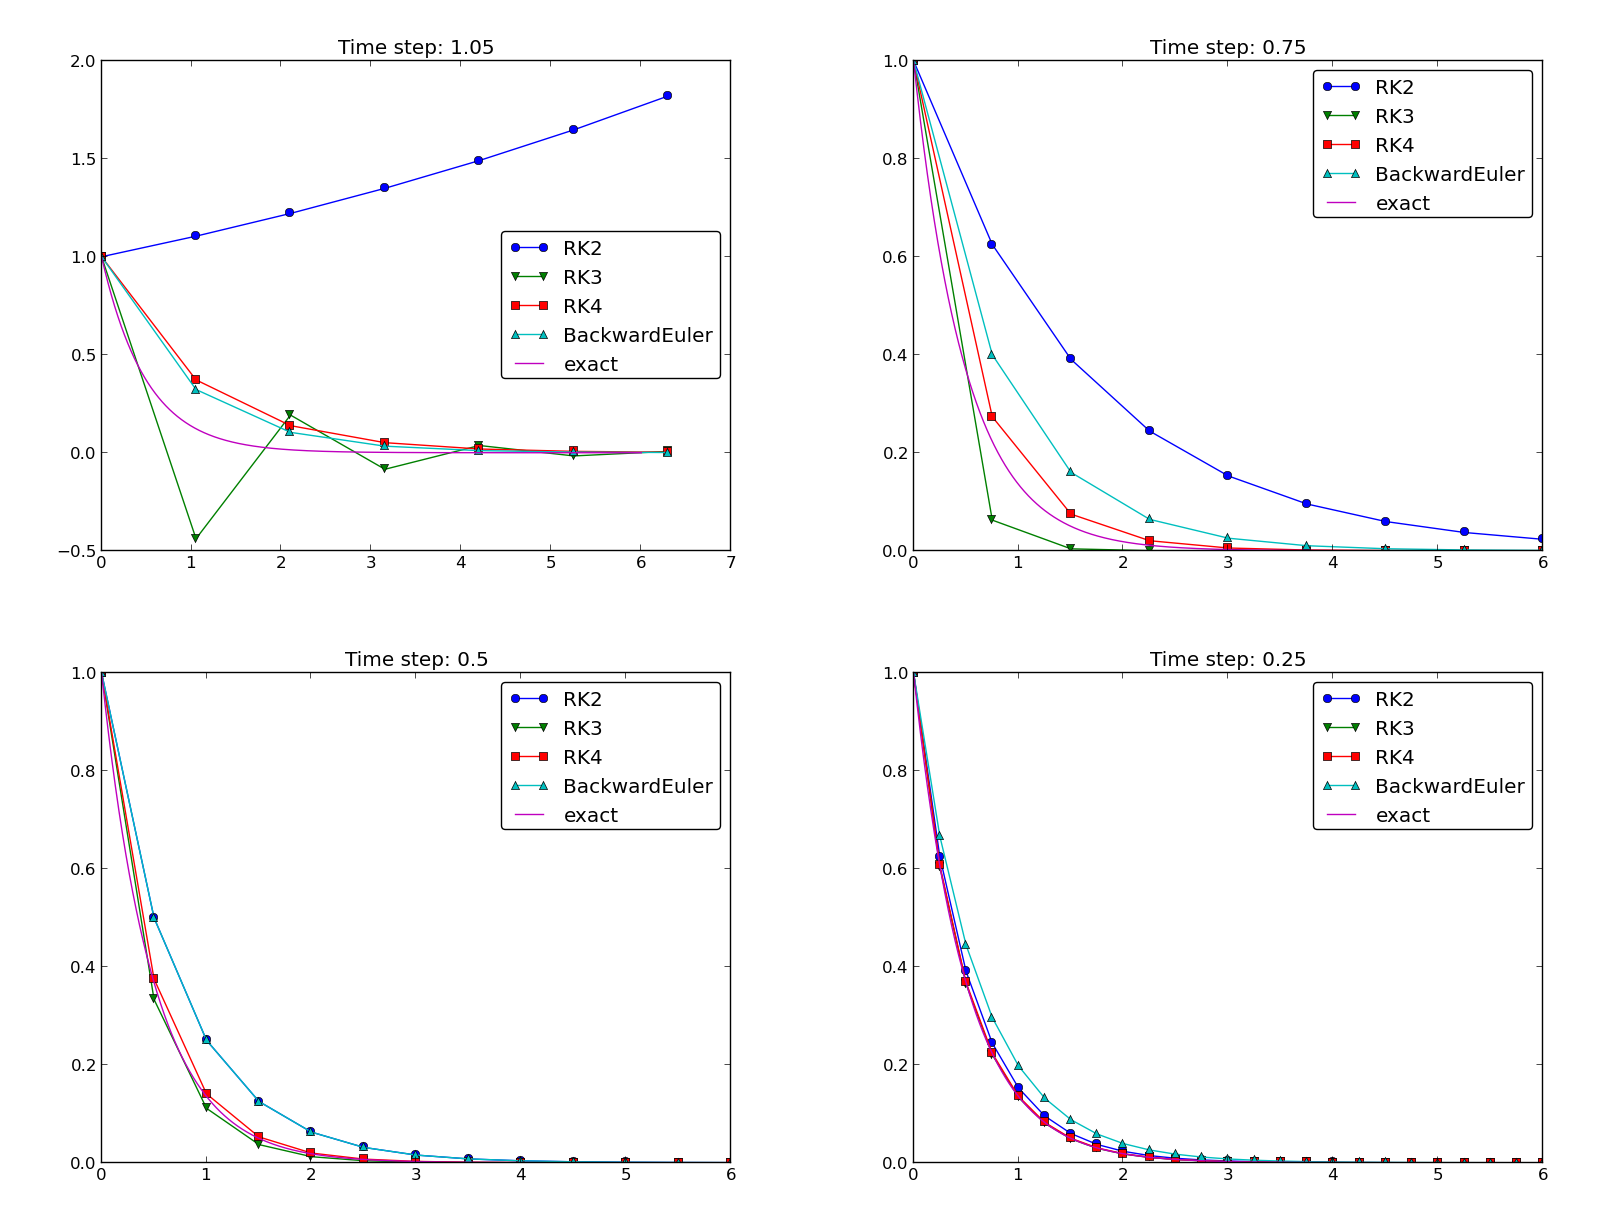
\includegraphics[width=0.9\linewidth]{fig-genz/decay_odespy1_png.png}}



The 4-th order Runge-Kutta method (\texttt{RK4}) is the method of choice!


% !split
\subsection*{Example: Adaptive Runge-Kutta methods}

\begin{itemize}
 \item Adaptive methods find "optimal" locations of the mesh points
   to ensure that the error is less than a given tolerance.

 \item Downside: approximate error estimation, not always optimal
   location of points.

 \item "Industry standard ODE solver": Dormand-Prince 4/5-th order
   Runge-Kutta (MATLAB's famous \texttt{ode45}).
\end{itemize}

\noindent
% inline figure
\centerline{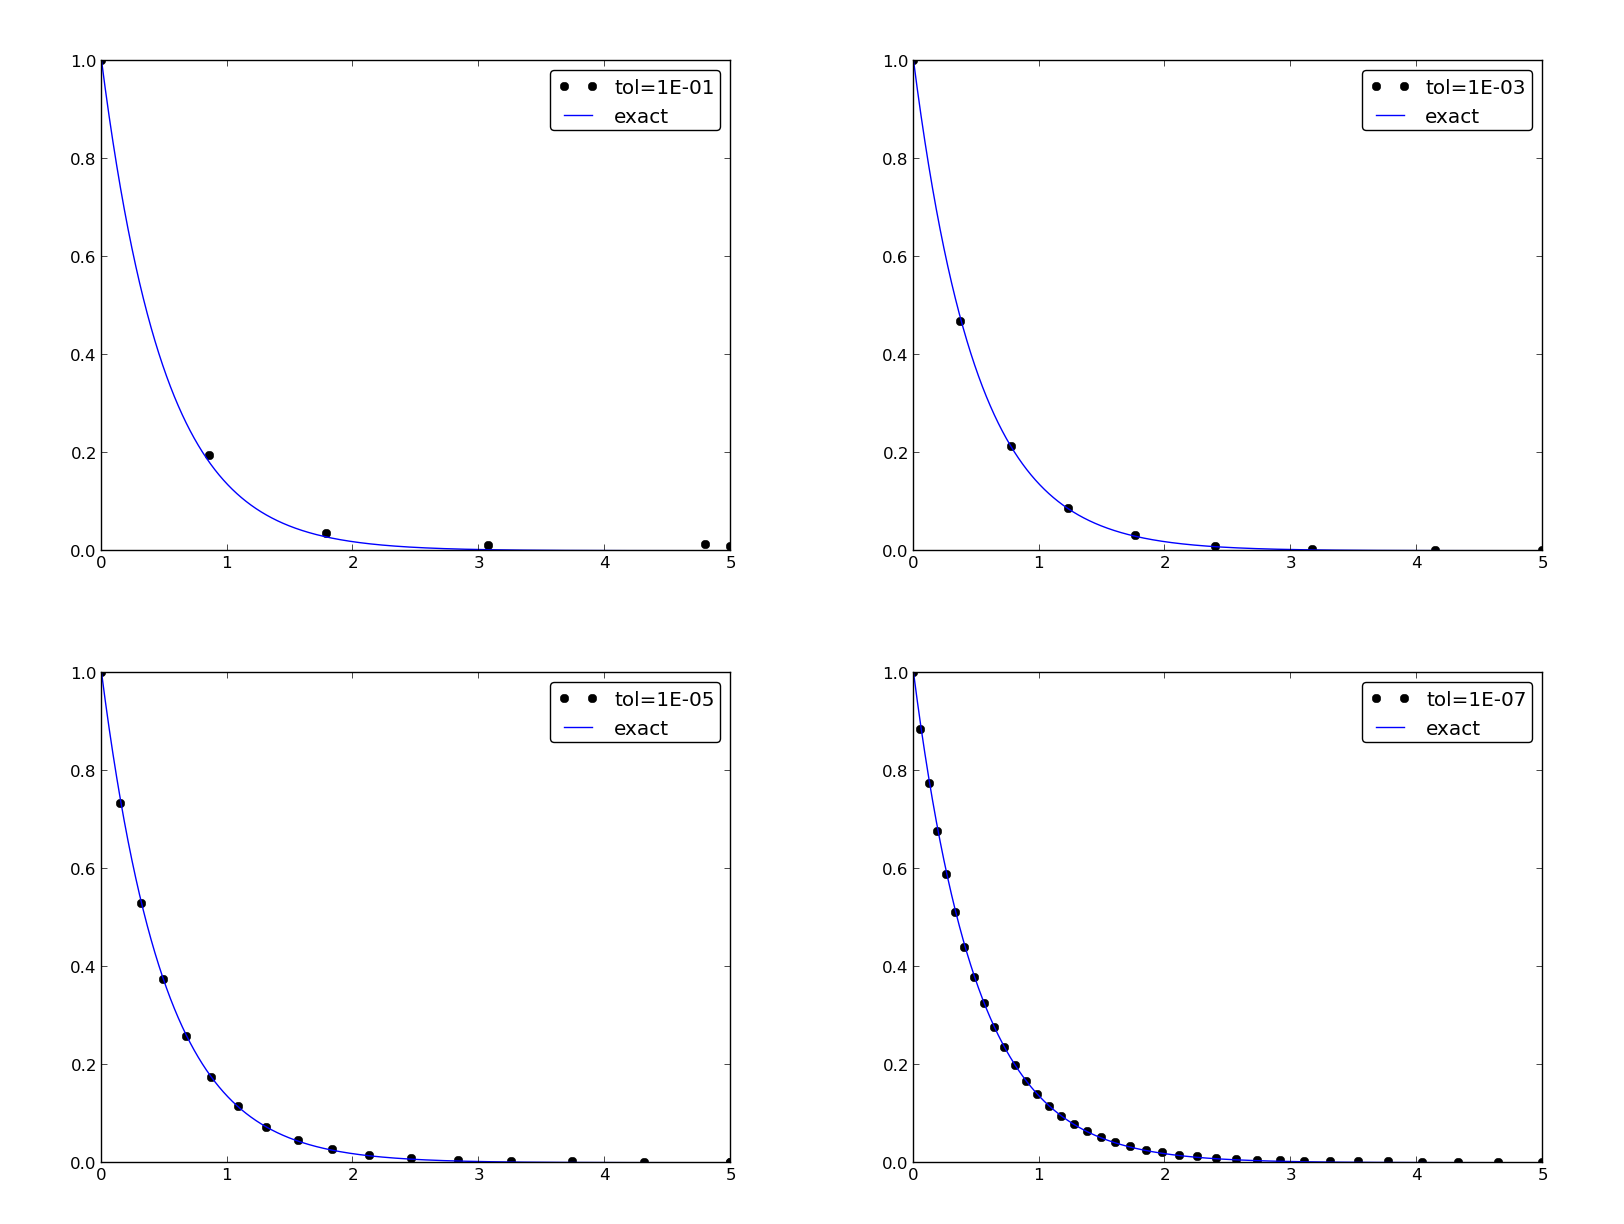
\includegraphics[width=0.9\linewidth]{fig-genz/decay_DormandPrince_adaptivity.png}}



% ------------------- end of main content ---------------

% #ifdef PREAMBLE
\cleardoublepage\phantomsection  % trick to get correct link to Index
\printindex

\end{document}
% #endif

